\newpage
\section{Circuitniveau}
\label{Circuit_niveau}
Voor het ontwikkelen van de applicatie is het nodig om de blokken uit het vereenvoudigde blokschema uit te gaan werken. Dit process wordt besproken in dit hoofdstuk. Als eerste wordt er gekeken naar de temperatuursensor.

\subsection{Temperatuursensor}
Voor het meten van temperatuur zijn er verschillende typen soorten op de markt. Om de correcte keuze te maken is het nodig om dit te vergelijken. In Figuur \ref{fig:verschillende_temp_sensors} zijn de verschillende typen sensoren weergegeven die veel in de industriële sector gebruikt wordt.

\begin{figure}[H]
    \centering
    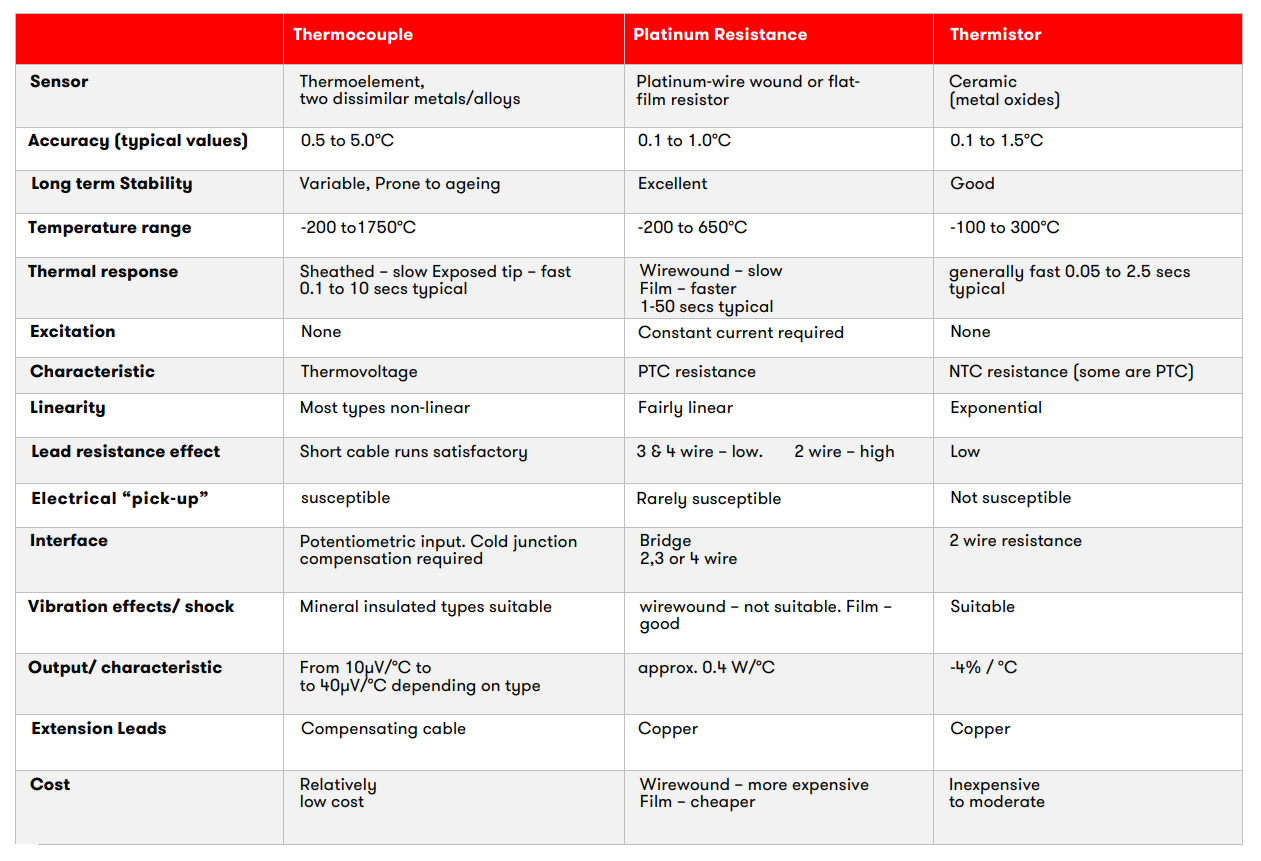
\includegraphics[width=1\linewidth]{pictures/RS_sensor_buyers_guide.png}
    \caption{Verschillende type temperatuur sensoren \cite{RS_temp_sensor}.}
    \label{fig:verschillende_temp_sensors}
\end{figure}

De specificaties hebben een nauwkeurigheid van 0.1 $^\circ\text{C}$ opgesteld. Hierdoor is het niet mogelijk om een thermokoppel te gebruiken. De andere twee optie halen wel de gespecificeerde temperatuur nauwkeurigheid van 0.1 $^\circ\text{C}$. Naast deze twee optie is er ook nog de optie van het zelf ontwikkelen van de sensor. Dit kan gedaan worden door middel van titaniumdraad. Dit komt doordat titanium net zoals platina een weerstand verandering heeft afhankelijk van temperatuur \cite{Titanium_temp_co}. Daarnaast heeft is titanium niet magnetische, wat ervoor zorgt dat het minder tot geen storing van buiten af oppikt. Hierdoor zou zelfs een beter nauwkeurigheid van 0.1 $^\circ\text{C}$ sensor ontwikkeld worden. Het probleem met titanium draad is de prijs. Hierdoor zal de sensor ontwikkelingskosten buiten het budget van dit vak gaan. Hierom is er niet gekozen voor deze keuze.  %hier ben ik nu met feedback verwerken

De keuze die er nu nog zijn de platina-weerstand en Thermistor. De reactie tijd van de Thermistor is lager dan die van de platina-weerstand.  Beide hebben een reactie tijd die binnen de eisen van de applicatie vallen. Hierom wordt er gekeken naar andere kwaliteiten van het type sensoren. Als er gekeken wordt naar de lineariteit van de sensor is te zien dat de Thermistor een exponentiële lineariteit heeft. Terwijl de platina-weerstand een redelijke lineaire uitgang heeft in vergelijk tot de temperatuur verandering. Hierdoor is het mogelijk om met de platina-weerstand een eenvoudiger Signaal versterking systeem te ontwikkelen. Hierdoor is er gekozen voor het gebruik van een platina-weerstand voor het ontwerpen van de Temperatuur sensor.
\\
\newline
Voor het gebruiken de platina-weerstand is er alleen een constant stroom bron nodig. 
Deze Stroombron mag niet tot zo min mogelijk temperatuur gevoelig zijn. Om de sensor minder nauwkeurig te maken. Dit kan bereikt worden door een Stroom bron te ontwikkelen met een lage ppm. Daarnaast moet de stroombron een stroom van tientallen $\mu$A leveren, zodat het systeem zo energie zuinig blijft. Zoals is weergegeven in Figuur \ref{fig:Stroombron_schema} en Tabel \ref{tab:stroom_bron_specs}.

\begin{figure}[H]
    \centering
    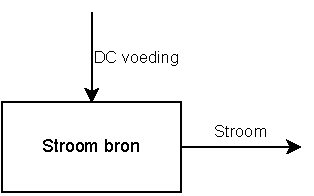
\includegraphics[width=0.5\linewidth]{pictures/Stroombron.drawio.pdf}
    \caption{Stroombron schema}
    \label{fig:Stroombron_schema}
\end{figure}

\begin{table}[H]
    \centering
    \caption{Specificaties van Stroombron voor de platina-weerstand}
    \begin{tabular}{|c|c|}
        \hline
        \textbf{Module} & \textbf{Stroombron} \\
        \hline
        \textbf{Ingangen} &  DC-voeding \\
        \hline
        \textbf{Uitgang(en)} & Stroom in $\mu$A \\
        \hline
        \textbf{Functie} & \begin{tabular}[c]{@{}c@{}}
        Zorgt voor een constante stroom die door de platina-weerstand gaat lopen\\
        Moet een lage PPM hebben om temperatuur onafhankelijk te zijn \\
        Heeft een minimale SNR van 60 dB
        \end{tabular} \\
        \hline
    \end{tabular}
    \label{tab:stroom_bron_specs}
\end{table}

\subsection{Signaal versterking}
De platina-weerstand heeft door de constante stroombron een spanningsverschil over hem heen staan. Om deze spanning te versterken is er een versterker nodig die van differentieel naar single ended  versterkt. Hiervoor zijn twee opamp implementatie mogelijk. De Differentiële versterker en Instrumentatie versterker. Hierin is de Instrumentatie een betere optie door hoge ingangsimpedantie en beter CMMR. Daarom is er gekozen voor een Instrumentatie versterking implementatie. De Schematische weergave van een Instrumentatie versterker in weergegeven in Figuur \ref{fig:instrumentatie_versterker_schematic}.

\begin{figure}[H]
    \centering
    
\includegraphics[width=0.5\linewidth]{pictures/instrumentatie_versterk.png}
    \caption{Schematische weergave van een Instrumentatie versterker \cite{Instrumentatie_versterker_schematic}.}
    \label{fig:instrumentatie_versterker_schematic}
\end{figure}

Nu de keuzes zijn gemaakt voor het type sensor en versterker is het mogelijk om een nieuw schema te maken waarin deze informatie verwerkt is. Dit schema is weergegeven in Figuur \ref{fig:Sensor_schematic_circuit_niveau}.

\begin{figure}[H]
    \centering
    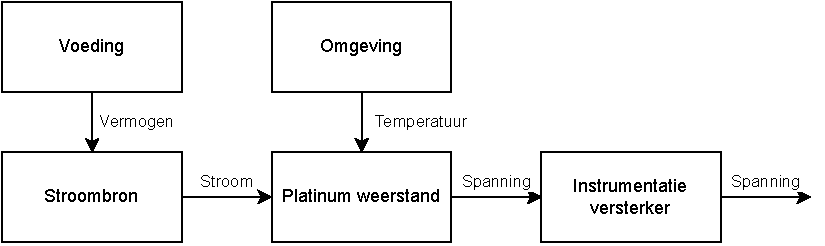
\includegraphics[width=0.8\linewidth]{pictures/Circuit_nivea_schema.drawio.pdf}
    \caption{De sensor en versterker blokken uitgewerkt.}
    \label{fig:Sensor_schematic_circuit_niveau}
\end{figure}

\newpage
\subsection{ADC} % dit in het blokschema niveau plaatsen
Het temperatuur bereik is van -5 tot 55 graden, om een nauwkeurigheid van 0.1 te halen zijn dus $\frac{60}{0.1}= 600$ stappen nodig. Dit betekent dat er minimaal een 10 bit adc nodig is. De reactie snelheid van de gekozen sensor is 1 tot 50 seconde, dit kan gebruikt worden om de minimale bemonstering frequentie te bepalen. Hiervoor wordt uitgegaan van de snelste tijd 1 seconde. Uitgaande van een maximale temperatuursverandering van -5 tot 55 graden. In 1 seconde reageert de sensor met ongeveer 63\% wat dus voor een maximale temperatuursverandering neerkomt op een stap van $0.63\cdot600 = 378$. Om elke veranderingsstap te kunnen meten zal dus een bemonsteringsfrequentie van minimaal 378 Hz nodig zijn.

\subsection{Digitale bewerking}
% Digitaal communicatie protocol nodig voor het uitlezen van luchtvochtigheid.


\subsection{DAC}
De data zal serieel verstuurd worden. Hierdoor is een 1 bit dac nodig, en hoeft dit eigenlijk niet meer echt een dac genoemd te worden, voor de implementatie hiervan betekent dit dat waarschijnlijk een gpio pin van een microcontroller al geschikt is.
\subsection{Zender}